\subsubsection{Merge Sort}

Figure \ref{fig:net_merge_sort} illustrates the time it takes for each language, run in the .NET environment, to sort one million randomly generated positive integers in ascending order.

\begin{figure}[h]
	\centering
	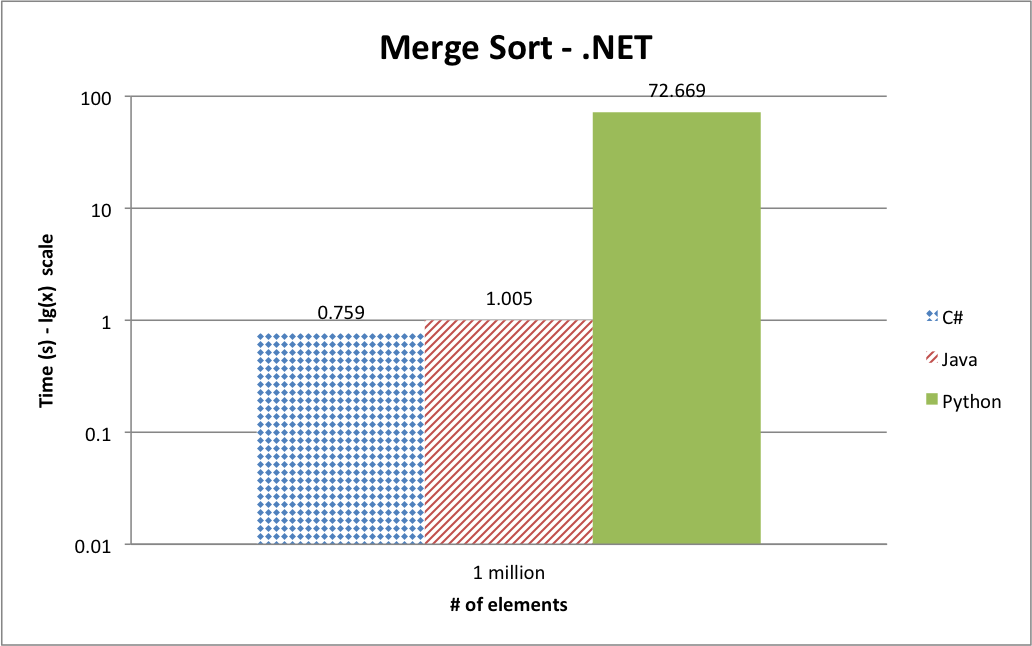
\includegraphics[width=1.0\linewidth]{chapters/new_media/MergeSortNet.png}
	\caption{This test is run in the .NET environment and uses the Merge sort algorithm to sort one million elements in ascending order. Lower is better. Note that the vertical axis is base 10 logarithmic. C\# is the fastest with 0.759 seconds. Java comes in second with 0.967 seconds. Python is the slowest with 71.663 seconds.}
	\label{fig:net_merge_sort}
\end{figure}

Figure \ref{fig:net_merge_sort_memory} illustrates the amount of MB used when running the merge sort algorithm in the .NET environment by the different languages.

\begin{figure}[h]
	\centering
	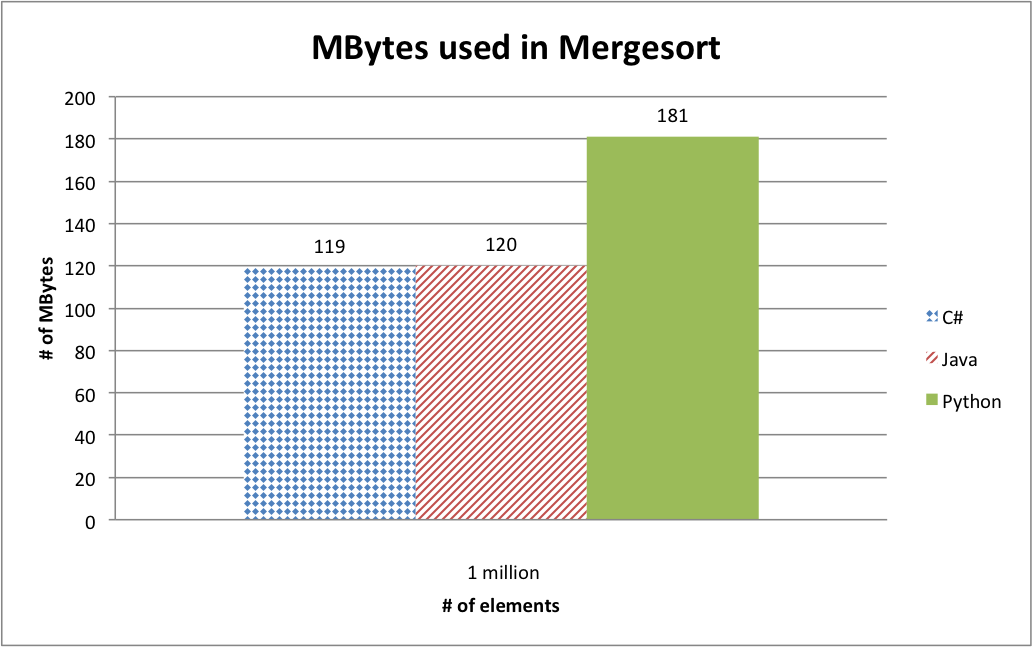
\includegraphics[width=1.0\linewidth]{chapters/new_media/MBytesMergesort.png}
	\caption{Add more text here...}
	\label{fig:net_merge_sort_memory}
\end{figure}
